\section{Analysis}

The hypothesis we are working with is that users having similar characteristics behave/interact similarly. Essentially, there are clusters of users that we can identify based on our input features. For the sake of this experiment, we decided to go with a simple clustering model, K-Means, using Euclidean distance as our distance metric. Our training dataset consisted of the control set of users which made up 10\% of our user base. We filtered for dense users within this to arrive at our final dataset. We concentrated on the dense users’ data as we were trying to replicate the dense user behavior onto similar sparse users. 



\subsection{Feature Engineering}

As a first step, we analyzed user's category preference and demographics data. Under demographic data, we had 4 features to work with: 

\begin{itemize}
    \item{\verb|gender of the user|}: a binary variable, identifying the predicted gender of the user 
    \item{\verb|tier of the city|}: a categorical variable having three values
    \item{\verb|price|}: a continuous variable, price of the Android phone
    \item{\verb|dpi|}: a continuous variable, screen resolution of the Android phone
\end{itemize}

Gender of the user was a derived feature based on various other device characteristics. For the continuous features such as price and dpi, we first bucketed them into defined ranges and encoded them as one-hot vectors. The tier of city and gender were similarly one-hot encoded. The user’s category preference comes as an 18-dimensional vector which we encoded as a multi-hot vector and normalized it. 




\subsection{Dimensionality Reduction}

On concatenating the normalized multi-hot category vector with the rest of the one-hot encoded features, our feature space was too large and sparse. Clustering the users via k-means clustering is unlikely to give meaningful clusters with such sparse and high dimensional data \cite{nur2015combination}. Here, Singular Value Decomposition (SVD) without mean normalization turned out to be the most suitable approach. To decide the optimal number of reduced dimensions, we plotted the inter and intra variance of the SVD matrix for a defined range of dimensions. The optimal dimension should have high inter variance (x-axis) and low intra variance (y-axis) scores, which came out to be 6 for us as shown in Figure \ref{fig:svd}.

\begin{figure}
  \centering
  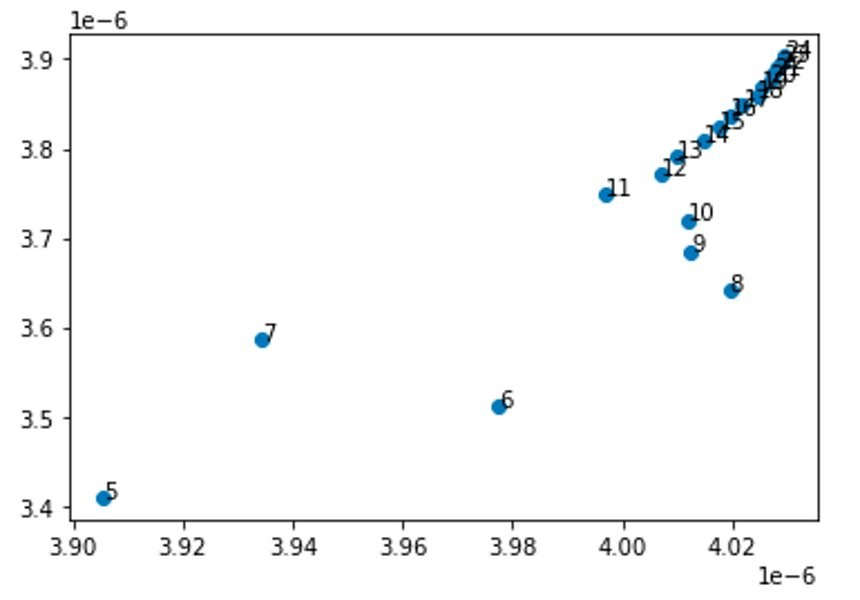
\includegraphics[width=\linewidth]{figures/svd_inter_intra.jpeg}
  \caption[Plot of inter-variance vs intra-variance]{Inter-variance (x-axis) vs intra-variance (y-axis) for SVD. The optimal number of dimensions comes out to be 6.}
  \label{fig:svd}
\end{figure}



\subsection{Finding optimal number of clusters}

We plotted an elbow graph for Within-Cluster Sum of Square (WCSS) \cite{bagirov2008modified} vs number of clusters to determine the optimal number of clusters for our clustering. WCSS is the sum of the squared distances between each point in a cluster and its centroid. As the number of cluster increases, the WCSS value decreases, giving us an elbow point where the WCSS value declines the most.  

The normalization of preference categories at a global level was not helping the model generalize, it was not calibrating the model for different user groups. We therefore incorporated the price of the device into the preference category vector, by normalizing the multi-hot category vector for each price bucket. Our reasoning here was that people buying devices in certain ranges would tend to have similar tastes. So, the preference categories vector now indicated how different the preferred categories were for a particular user as compared to other users in the same price bucket of the device.  

This helped us greatly in tuning the model. After all the iterations, the optimal number of clusters came out to be 6, as evidenced by the faint elbow in Figure \ref{fig:elbow}.

\begin{figure}
  \centering
  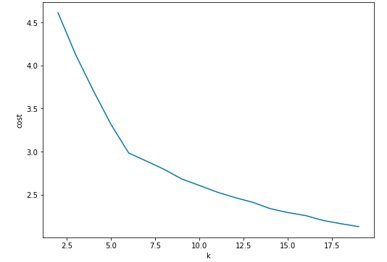
\includegraphics[width=\linewidth]{figures/elbow.jpeg}
  \caption[Elbow curve to identify optimum cluster number]{Plot of the elbow curve, WCSS vs number of clusters. The optimal number of clusters comes out to be 6.}
  \label{fig:elbow}
\end{figure}

On checking the feature distributions of the clusters, we were able to see clear distinctions, which meant that we had meaningful clusters. The distinction was clear enough to engineer user personas out of it, reproduced in Table \ref{tab:persona}.

\begin{table*}
  \caption{User personas emerging out of the clusters}
  \label{tab:persona}
  \begin{tabular}{llllll}
    \toprule
    Cluster&DPI&Tier&Gender&Price&Preference Categories (ordered by priority)\\
    \midrule
    0 & High & Mix & Male & Mix & Finance, Productivity, Entertainment\\
    1 & High & T1 \& T3 & Dominant Male & Mix & Shopping, Finance, Business, Social\\
    2 & High & Mix & Dominant Male & Middle & Finance, Social\\
    3 & Very Low & Mix & Mix & Low & Finance, Social, Entertainment\\
    4 & Low & Mix & Mix & Middle & Social, Entertainment, Finance, Shopping\\
    5 & Very High & Mix & Mix & High & Shopping, Finance, Entertainment, Productivity\\
  \bottomrule
\end{tabular}
\end{table*}



\subsection{Correlating with interaction data}

Our immediate next step was to check how well these clusters relate to the user’s interactions. More precisely, we wanted the users of these clusters to have different behaviors. For our dense users clustered in our training dataset, we looked at their interaction scores over a 30-day period. These interactions were calculated over a binary set of rewards, given when a user positively interacts with Bubbles. The scores were aggregated for the categories of the Bubbles interacted by the user, and then aggregated again at a cluster level. We thus prepared a weight matrix, which is the mapping between cluster numbers and mean interaction score of categories, for the users in those clusters. 

\begin{figure*}
  \centering
  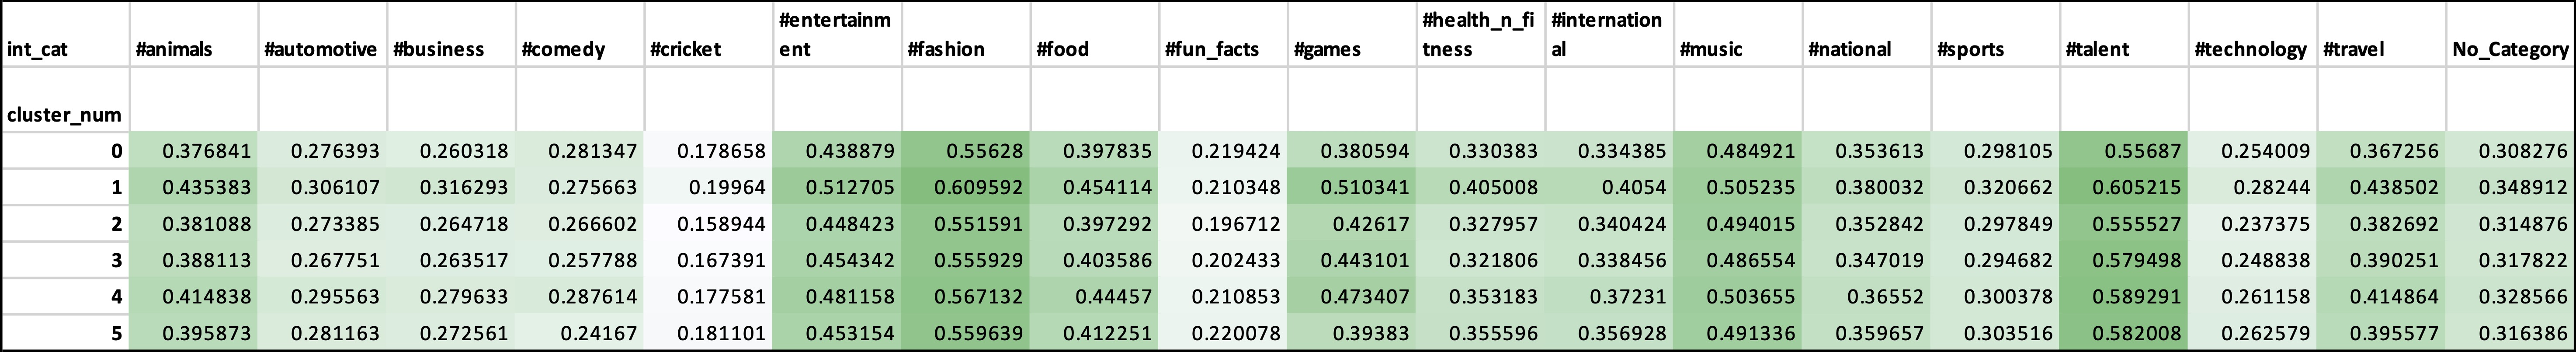
\includegraphics[width=\linewidth]{figures/mean_weight_matrix.jpg}
  \caption[Mean Weight Matrix]{A map of cluster number and the mean interaction score of the users belonging to the cluster}
  \label{fig:mean_weight_matrix}
\end{figure*}

Figure \ref{fig:mean_weight_matrix} represents this mean weight matrix. Here, the vertical bands mean that all the clusters behave generally similarly across the interaction categories. The very slight horizontal banding means there is a variation in the interaction behavior. But that was too slight a variation to have any predictive power.  

\begin{figure*}
  \centering
  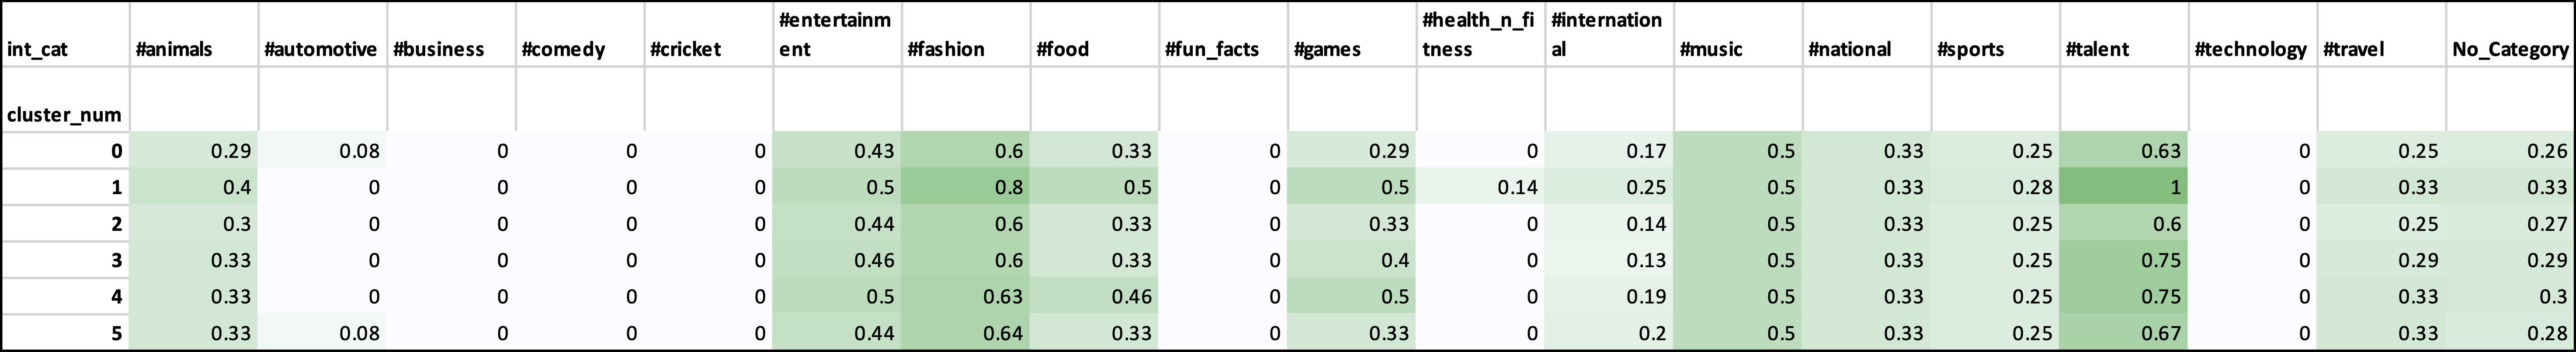
\includegraphics[width=\linewidth]{figures/median_weight_matrix.jpg}
  \caption[Median Weight Matrix]{A map of cluster number and the median interaction score of the users belonging to the cluster}
  \label{fig:median_weight_matrix}
\end{figure*}

Since mean interaction scores were possibly skewed due to outliers, we repeated the same exercise with median interaction scores and now the horizontal banding became more distinct, as shown in Figure \ref{fig:median_weight_matrix}. Notice how cluster 1 and 4 stand out generally in all categories, 0 and 5 in automotive, and cluster 1 in health and fitness. This highlighted a correlation between the clusters and the interaction categories that could be leveraged for sparse users’ recommendation.

